% created on 28/07/2020
% @author : ebazan
\part{Global Color and Texture}\label{part:global_color_texture}%Image Global Color and Texture

\section*{Introduction}
In part \ref{part:image_contours}, we show that low-level features, such as image contours, provide useful perceptual information that can be used to solve complex problems. We presented a framework that uses the concepts of human perception and contour information for the unsupervised detection of landing targets. This framework is able to identify the marker under degraded operating conditions using only exogenous features from the contours, which are identified on gray-level images. The framework can be improved by adding other features that provide perceptual information of a scene.

In this part of the thesis, we review two more low-level image features: color and texture. Both features are widely involved in the perceptual process of humans and their study can be very extensive. The objective of this part is to explore the image color and texture features for their future integration into a general framework for object detection. Particularly, in this part of the thesis we are interested in the global distribution of color and texture information of an image. For this purpose, the chapter that opens this part seeks to remember recall the definition of color and texture in the field of computer vision. Moreover, it review different approaches to color representation as well as different strategies for characterizing texture features. Later, in chapter \ref{ch:similarity_measures}, we take interest at the comparison of distributions, particularly in the study of the Optimal Transport (OT) as a metric for the measurement of similarity between distributions and its application in the field of computer vision.

Throughout these chapters of the thesis, we address the study of those two properties using simple images containing the information of interest; in the case of color, images containing low color variation and; in the case of texture, grayscale images with homogeneous textures.

The main contributions of this part are:

\begin{enumerate}
	\item Review of the state of the art of global color representations and texture characterizations.
	\item Review of the state of the art of similarity measures, particulary the interpretation of the OT in computer vision: the Earth Mover's Distance (EMD).
	\item Qualitative and quantitative study between the most popular measures in the comparison of distributions and the EMD. 
	\item An unsupervised image retrieval system based on global color/texture information.
\end{enumerate}


\chapter{Global Representations of Color and Texture } \label{ch:color_texure_representations}

\section*{Résumé}
\noindent 
Ce chapitre présente une compilation des différentes manières de représenter les informations de couleur et de texture présentes dans une image. En ce qui concerne les informations de couleur, nous introduisons certains types d'espaces colorimétriques et leurs origines. De plus, nous présentons quelques techniques pour synthétiser ces informations. Dans le cas de la texture, nous présentons les différentes méthodologies pour son étude, en mettant en évidence les avantages et les inconvénients de chaque méthode.
\section*{Abstract}
\noindent 
This chapter presents a compilation of the different ways of representing the color and texture information present in an image. When it comes to color information, we present some of the most popular color spaces used as well as their origins and relationship to human perception. In addition, we present some techniques to synthesize this information. In the case of texture, we present the different methodologies for its study, highlighting the advantages and disadvantages of each method. The information presented in this chapter serves as the basis for the next chapter.

\section{Introduction}

If we look around us, we can see that many of the materials and objects of our environment only exist with certain colors. For example, the clouds are mostly  white, the grass is green, the ocean is blue, etc. Performing the same experience, but this time with textures, we realize that we are surrounded by them everywhere. We find textures, for example, at textiles, buildings, tilings and on skins or objects surfaces. The color and texture of an image is very valuable information and therefore, the perception of such information is a powerful tool for classifying and recognizing certain objects and materials.

For decades several vision algorithms have sought to exploit this information. Color and texture are of relevant importance for its use as a feature to characterize objects. Due to these facts, the definition and the various representations of the color, as well as the texture information, is addressed in this chapter. As far as color information is concerned, we give a brief introduction to what color is and how it can be represented. In the case of texture, we present a brief introduction to textures including its types and an overview to the various methodologies for its study, highlighting the advantages and disadvantages of each method. 


\begin{figure}[!ht]
    \centering
    \begin{subfigure}[b]{0.24\textwidth}
        \includegraphics[width=\textwidth]{tempo}
        \caption{}
        \label{fig:tempo}
    \end{subfigure}
    %~ %add desired spacing between images, e. g. ~, \quad, \qquad, \hfill etc. 
      %(or a blank line to force the subfigure onto a new line)
    \begin{subfigure}[b]{0.24\textwidth}
        \includegraphics[width=\textwidth]{mountain}
        \caption{}
        \label{fig:parrots}
    \end{subfigure} 
    %~ %add desired spacing between images, e. g. ~, \quad, \qquad, \hfill etc. 
      %(or a blank line to force the subfigure onto a new line)    
    \begin{subfigure}[b]{0.24\textwidth}
        \includegraphics[width=\textwidth]{clownfish}
        \caption{}
        \label{fig:clownfish}
    \end{subfigure}
    %~ %add desired spacing between images, e. g. ~, \quad, \qquad, \hfill etc. 
      %(or a blank line to force the subfigure onto a new line)
    \begin{subfigure}[b]{0.24\textwidth}
        \includegraphics[width=\textwidth]{araras}
        \caption{}
        \label{fig:mountains}
    \end{subfigure}
                  
    \caption{Some examples of color images: One synthetic image {\small \textsf{\textbf{(a)}}} and three natural images [{\small \textsf{\textbf{(b) (c) (d)}}}].}\label{fig:color_images}    
\end{figure}


\section{Color}

Color is a physical property linked to the electromagnetic spectrum of light \citep{Beyerer.Leon.ea:Book:2016}. The perception of color in humans results from the quantity and wavelength captured by the eyes. This perception depends on many factors such as the type of surfaces or objects where the light is reflected, the environment and even the eyes of the observer. The perception of color is then an entirely arbitrary creation of our nervous system, and there is no way it is contained in the wavelengths or in light-reflecting objects and materials \citep{Goldstein:Book:2009} \citep{Beyerer.Leon.ea:Book:2016}. When an incident spectrum contains all frequencies in the range of visible wavelengths, humans perceive objects that reflect all frequencies as clear or \textit{white}. In the opposite case, when the material absorbs and does not reflect the visible frequencies, it is perceived as dark or \textit{black} {Gonzalez.Woods:Book:2008}. 

Although color has measurable physical properties, the interpretation and perception of this information is completely subjective. A clear example of this is the naming of colors. Some works in this regard state that the naming of colors varies according to culture and language \citep{Berlin.Kay:Book:1991}. However, it is possible to find a correlation between languages and identify eleven basic color terms in English language that  seem to be anchored across the different languages as points in a certain color space \citep{Kay.Regier:PNAS:2003}. The definition of a coherent color space to the final task is therefore essential to represent the color information digitally.


\section{Color representation}

The representation of color has evolved over time developing theories, such as the trichromatic theory or the opponent-colors theory \citep{Fairchild:Book:2005}, that attempt to explain the function of color vision. The result of these theories has been the development of abstract mathematical models that serve to represent colors as vectors or tuples of numbers. These vectors, which are mostly in three dimensions, can be arranged in a variety of ways. Such particular organizations are known as color models.

One of the main contributors in the creation of color spaces is the \textit{Commission Internationale de l'Éclairage} (CIE) \citep{CIE:Journal:1932}, who defined the three standard primaries of color $X$, $Y$ and $Z$. These primaries allow to define any visible color of the spectrum (see figure \ref{fig:visual_spectrum}) as a weighted sum of the three primary colors. They are defined mathematically with positive color-matching functions that specify the amount of each primary needed to describe any spectral color \citep{Wright:BookCh2:2007}. This color model is known as the CIE 1931 XYZ.

The \textbf{XYZ color model} quantify an object’s color using a standardized method taking into account the human eye’s (observer) response to these colors in the calculation. $X$, $Y$ and $Z$ are the amount of each primary needed to produce a desired color
\begin{eqnarray} 
 C(\lambda) = (X,Y,Z) \label{eq:g_energy}
\end{eqnarray}
where the primary $Y$ is chosen such that its colour-matching function exactly matches the luminous-efficiency function for the human eye \citep{Wright:BookCh2:2007}. Therefore, to define a color in this space, we need to provide the weights fot the $X$, $Y$ and $Z$ primaries, for example, color $=xX + yY + zZ$. 
 

\begin{figure}[!ht]
    \centering
    \begin{subfigure}[b]{0.45\textwidth}
        \includegraphics[width=\textwidth]{CIE_visible_spectrum}
        \caption{}
        \label{fig:visual_spectrum}
    \end{subfigure}
    %~ %add desired spacing between images, e. g. ~, \quad, \qquad, \hfill etc. 
      %(or a blank line to force the subfigure onto a new line)
    \begin{subfigure}[b]{0.45\textwidth}
        \includegraphics[width=\textwidth]{CIE_chromaticity_diagram}
        \caption{}
        \label{fig:chrom_diagram}
    \end{subfigure} 
                      
    \caption{CIE 1931 2 Degree Standard Observer: visible light spectrum {\small \textsf{\textbf{(a)}}} and chromaticity diagram {\small \textsf{\textbf{(b)}}}.}\label{fig:cie_standard_observer}    
\end{figure}


The \textbf{RGB color model} According to the three-component theory, our eyes only respond three primary colors of light; red, green, and blue . This theory gave rise to one of the first color models, which says that nearly all colors in the visible spectrum could be generated from the mixture of these three primaries (e.g. combining red and green produces yellow)\citep{Goldstein:Book:2009}. This occurs mainly because the red, green, and blue primaries of this color model are not standarized. 







\textbf{HSV color model}

\textbf{HSL color model}

\textbf{LAB color model} (also known as CIEL*a*b* or CIELAB)


\begin{itemize}

	\item \textbf{RBG (Red-Green-Blue)} A color space that maps the amount of red, green and blue light perceived to reproduce the visible color gamut.
	\item \textbf{HSV (Hue-Saturation-Value) and HSL (Hue-Saturation-Lightness)} Alternative representations to the RGB color space that more closely aligns with the way human vision perceives color-creating attributes.
	\item \textbf{Lab (CIEL*a*b*) / Luv (CIEL*u*v*).} A color space where L compenent represents luminance and a* and b* (resp. u* v*) components represent chroma. This representation was created to reflect the high sensitivity of humans to changes in luminance in the perception of color.
\end{itemize}


\begin{figure}[!ht]
    \begin{subfigure}[t]{\dimexpr0.3\textwidth+20pt\relax}
    	\makebox[20pt]{\raisebox{35pt}{ \rotatebox[origin=c]{90} {\small \textsf{\textbf{Input image}}} }}%
    	\includegraphics[width=\dimexpr\linewidth-20pt\relax]{araras}
    \end{subfigure} \\    
     
    \begin{subfigure}[t]{\dimexpr0.3\textwidth+20pt\relax}
    	\makebox[20pt]{\raisebox{35pt}{ \rotatebox[origin=c]{90} {\small \textsf{\textbf{RGB channels}}} }}%
    	\includegraphics[width=\dimexpr\linewidth-20pt\relax]{araras_R}
    \end{subfigure}      
    ~ %add desired spacing between images, e. g. ~, \quad, \qquad, \hfill etc. 
      %(or a blank line to force the subfigure onto a new line)
    \begin{subfigure}[b]{0.3\textwidth}
        \includegraphics[width=\textwidth]{araras_G}
    \end{subfigure}
    ~ %add desired spacing between images, e. g. ~, \quad, \qquad, \hfill etc. 
      %(or a blank line to force the subfigure onto a new line)
    \begin{subfigure}[b]{0.3\textwidth}
        \includegraphics[width=\textwidth]{araras_B}
    \end{subfigure} \vspace{5pt}      
    
    \begin{subfigure}[t]{\dimexpr0.3\textwidth+20pt\relax}
    	\makebox[20pt]{\raisebox{35pt}{ \rotatebox[origin=c]{90} {\small \textsf{\textbf{HSV channels}}} }}%
    	\includegraphics[width=\dimexpr\linewidth-20pt\relax]{araras_H}
    \end{subfigure}     
    ~ %add desired spacing between images, e. g. ~, \quad, \qquad, \hfill etc. 
      %(or a blank line to force the subfigure onto a new line)
    \begin{subfigure}[b]{0.3\textwidth}
        \includegraphics[width=\textwidth]{araras_S}
    \end{subfigure}
    ~ %add desired spacing between images, e. g. ~, \quad, \qquad, \hfill etc. 
      %(or a blank line to force the subfigure onto a new line)
    \begin{subfigure}[b]{0.3\textwidth}
        \includegraphics[width=\textwidth]{araras_V}
    \end{subfigure} \vspace{5pt}  
        
    \begin{subfigure}[t]{\dimexpr0.3\textwidth+20pt\relax}
    	\makebox[20pt]{\raisebox{35pt}{ \rotatebox[origin=c]{90} {\small \textsf{\textbf{LAB channels}}} }}%
    	\includegraphics[width=\dimexpr\linewidth-20pt\relax]{araras_L}
    \end{subfigure}    
    ~ %add desired spacing between images, e. g. ~, \quad, \qquad, \hfill etc. 
      %(or a blank line to force the subfigure onto a new line)
    \begin{subfigure}[b]{0.3\textwidth}
        \includegraphics[width=\textwidth]{araras_a}
    \end{subfigure}
    ~ %add desired spacing between images, e. g. ~, \quad, \qquad, \hfill etc. 
      %(or a blank line to force the subfigure onto a new line)
    \begin{subfigure}[b]{0.3\textwidth}
        \includegraphics[width=\textwidth]{araras_b}
    \end{subfigure} 

	\caption{Color channels of an image in different color spaces in a grayscale}\label{fig:images_color_space}    
\end{figure}

The overall distribution of color within an image is a useful clue that contributes to the description of the content of an image. For example, we can characterize images that contain landscapes with mountains, jungles, urban environments, deserts or other scenes with different elements by their color distribution. The global color distribution can be represented by means of a color image histogram, which is a discrete function that associates to each intensity value (per color channel) the number of pixels that belong to this value.

The advantages of this representation is that they are invariant to the rotation or translation of the image, as well as, to a lesser extent, to changes of point of view and changes of scale. In addition, we can compact the image color information by reducing the count intervals, that is, by selecting a small number of bins.

\subsection{Single-channel Color Histogram}

\begin{figure}[!ht]
    \centering
    \begin{subfigure}[b]{0.45\textwidth}
        \includegraphics[width=\textwidth]{araras}
        \caption{Input image}
    \end{subfigure}
        ~ %add desired spacing between images, e. g. ~, \quad, \qquad, \hfill etc. 
      %(or a blank line to force the subfigure onto a new line)
    \begin{subfigure}[b]{0.45\textwidth}
        \includegraphics[width=\textwidth]{araras_single_histogram}
        \caption{Single-channel color pixel distribution}
    \end{subfigure} 
    
    \caption{}\label{fig:single_channel_histogram}    
\end{figure}
    
    
\subsection{3-d Color Histogram}

\begin{figure}[!ht]
    \centering
    \begin{subfigure}[b]{0.4\textwidth}
        \includegraphics[width=\textwidth]{araras}
        \caption{Input image}
    \end{subfigure} \\
       
    \begin{subfigure}[b]{0.49\textwidth}
        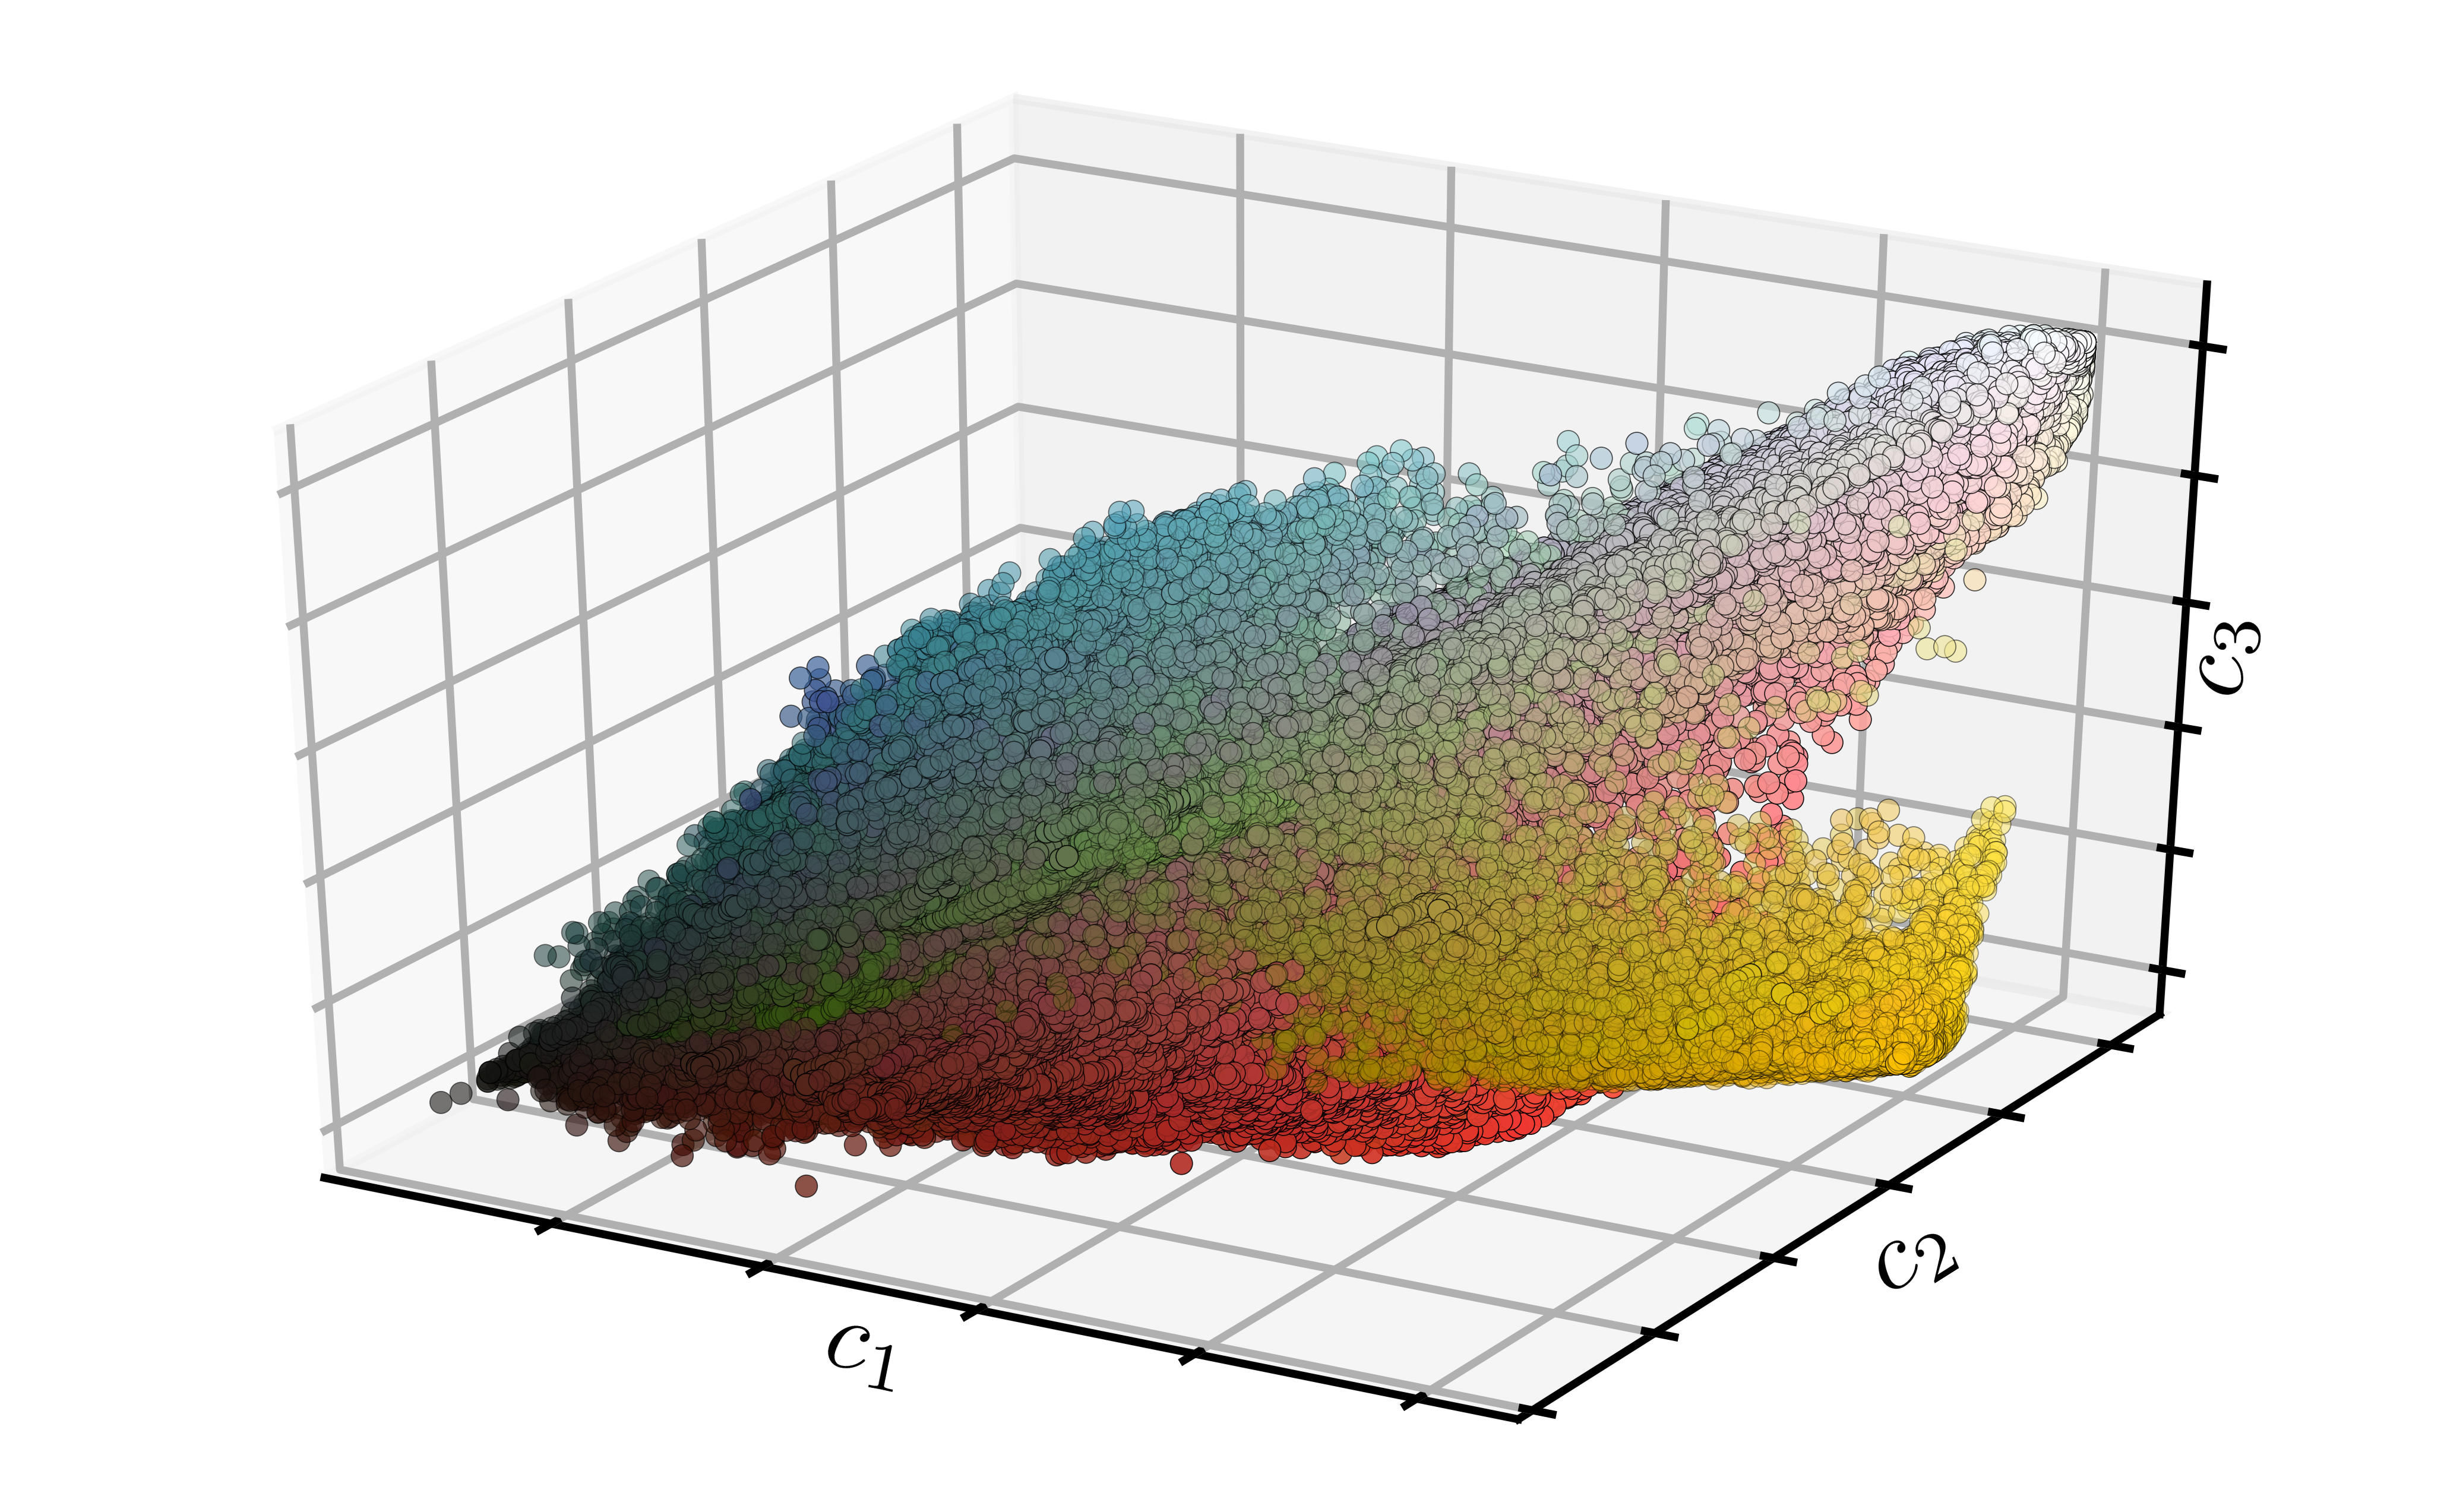
\includegraphics[width=\textwidth]{araras_3d_distribution}
        \caption{3-d image color pixel distribution}
    \end{subfigure} 
    \begin{subfigure}[b]{0.49\textwidth}
        \includegraphics[width=\textwidth]{araras_3d_histogram}
        \caption{3-d color pixel histogram}
    \end{subfigure} 
    
    \caption{3-d image color representation. 3-d pixel distribution and 10 bins 3-d pixel histogram.}\label{fig:3d_color_representation}    
\end{figure}


\subsection{Color Signature}

\begin{figure}[!ht]
    \centering
    \begin{subfigure}[b]{0.4\textwidth}
        \includegraphics[width=\textwidth]{araras}
        \caption{Input image}
    \end{subfigure} \\
    
    \begin{subfigure}[b]{0.4\textwidth}
    	\includegraphics[width=\textwidth]{araras_color_clusters}
        \includegraphics[width=\textwidth]{araras_bar_signature}
        \caption{Color signature}
    \end{subfigure}
    	~ %add desired spacing between images, e. g. ~, \quad, \qquad, \hfill etc. 
      %(or a blank line to force the subfigure onto a new line)
    \begin{subfigure}[b]{0.5\textwidth}
        \includegraphics[width=\textwidth]{araras_3d_signature}
        \caption{3-d representation of color ignature}
    \end{subfigure} 
    	    
    \caption{Image color signature and the 3-d visualization of signature clusters.}\label{fig:color_signature}    
\end{figure}



\begin{figure}[!ht]
    \centering
    \begin{subfigure}[t]{\dimexpr0.32\textwidth+20pt\relax}
    	\makebox[20pt]{\raisebox{40pt}{ \small\textbf{\textsf{(a)}} }}%
    	\includegraphics[width=\dimexpr\linewidth-20pt\relax]{tempo}
    \end{subfigure}~ 
%    \begin{subfigure}[b]{0.32\textwidth}
%        \includegraphics[width=\textwidth]{araras}
%    \end{subfigure}~
    \begin{subfigure}[b]{0.32\textwidth}
        \includegraphics[width=\textwidth]{clownfish}
    \end{subfigure}~
    \begin{subfigure}[b]{0.32\textwidth}
        \includegraphics[width=\textwidth]{mountain}
    \end{subfigure}\vspace{10pt}
    
    \begin{subfigure}[t]{\dimexpr0.32\textwidth+20pt\relax}
    	\makebox[20pt]{\raisebox{40pt}{ \small\textbf{\textsf{(b)}} }}%
    	\includegraphics[width=\dimexpr\linewidth-20pt\relax]{tempo_single_histogram}
    \end{subfigure}~     
%    \begin{subfigure}[b]{0.32\textwidth}
%        \includegraphics[width=\textwidth]{araras_single_histogram}
%    \end{subfigure}~
    \begin{subfigure}[b]{0.32\textwidth}
        \includegraphics[width=\textwidth]{clownfish_single_histogram}
    \end{subfigure}~
    \begin{subfigure}[b]{0.32\textwidth}
        \includegraphics[width=\textwidth]{mountain_single_histogram}
    \end{subfigure}\vspace{10pt}
    
    \begin{subfigure}[t]{\dimexpr0.32\textwidth+20pt\relax}
    	\makebox[20pt]{\raisebox{40pt}{ \small\textbf{\textsf{(c)}} }}%
    	\includegraphics[width=\dimexpr\linewidth-20pt\relax]{tempo_3d_distribution}
    \end{subfigure}~ 
%    \begin{subfigure}[b]{0.32\textwidth}
%        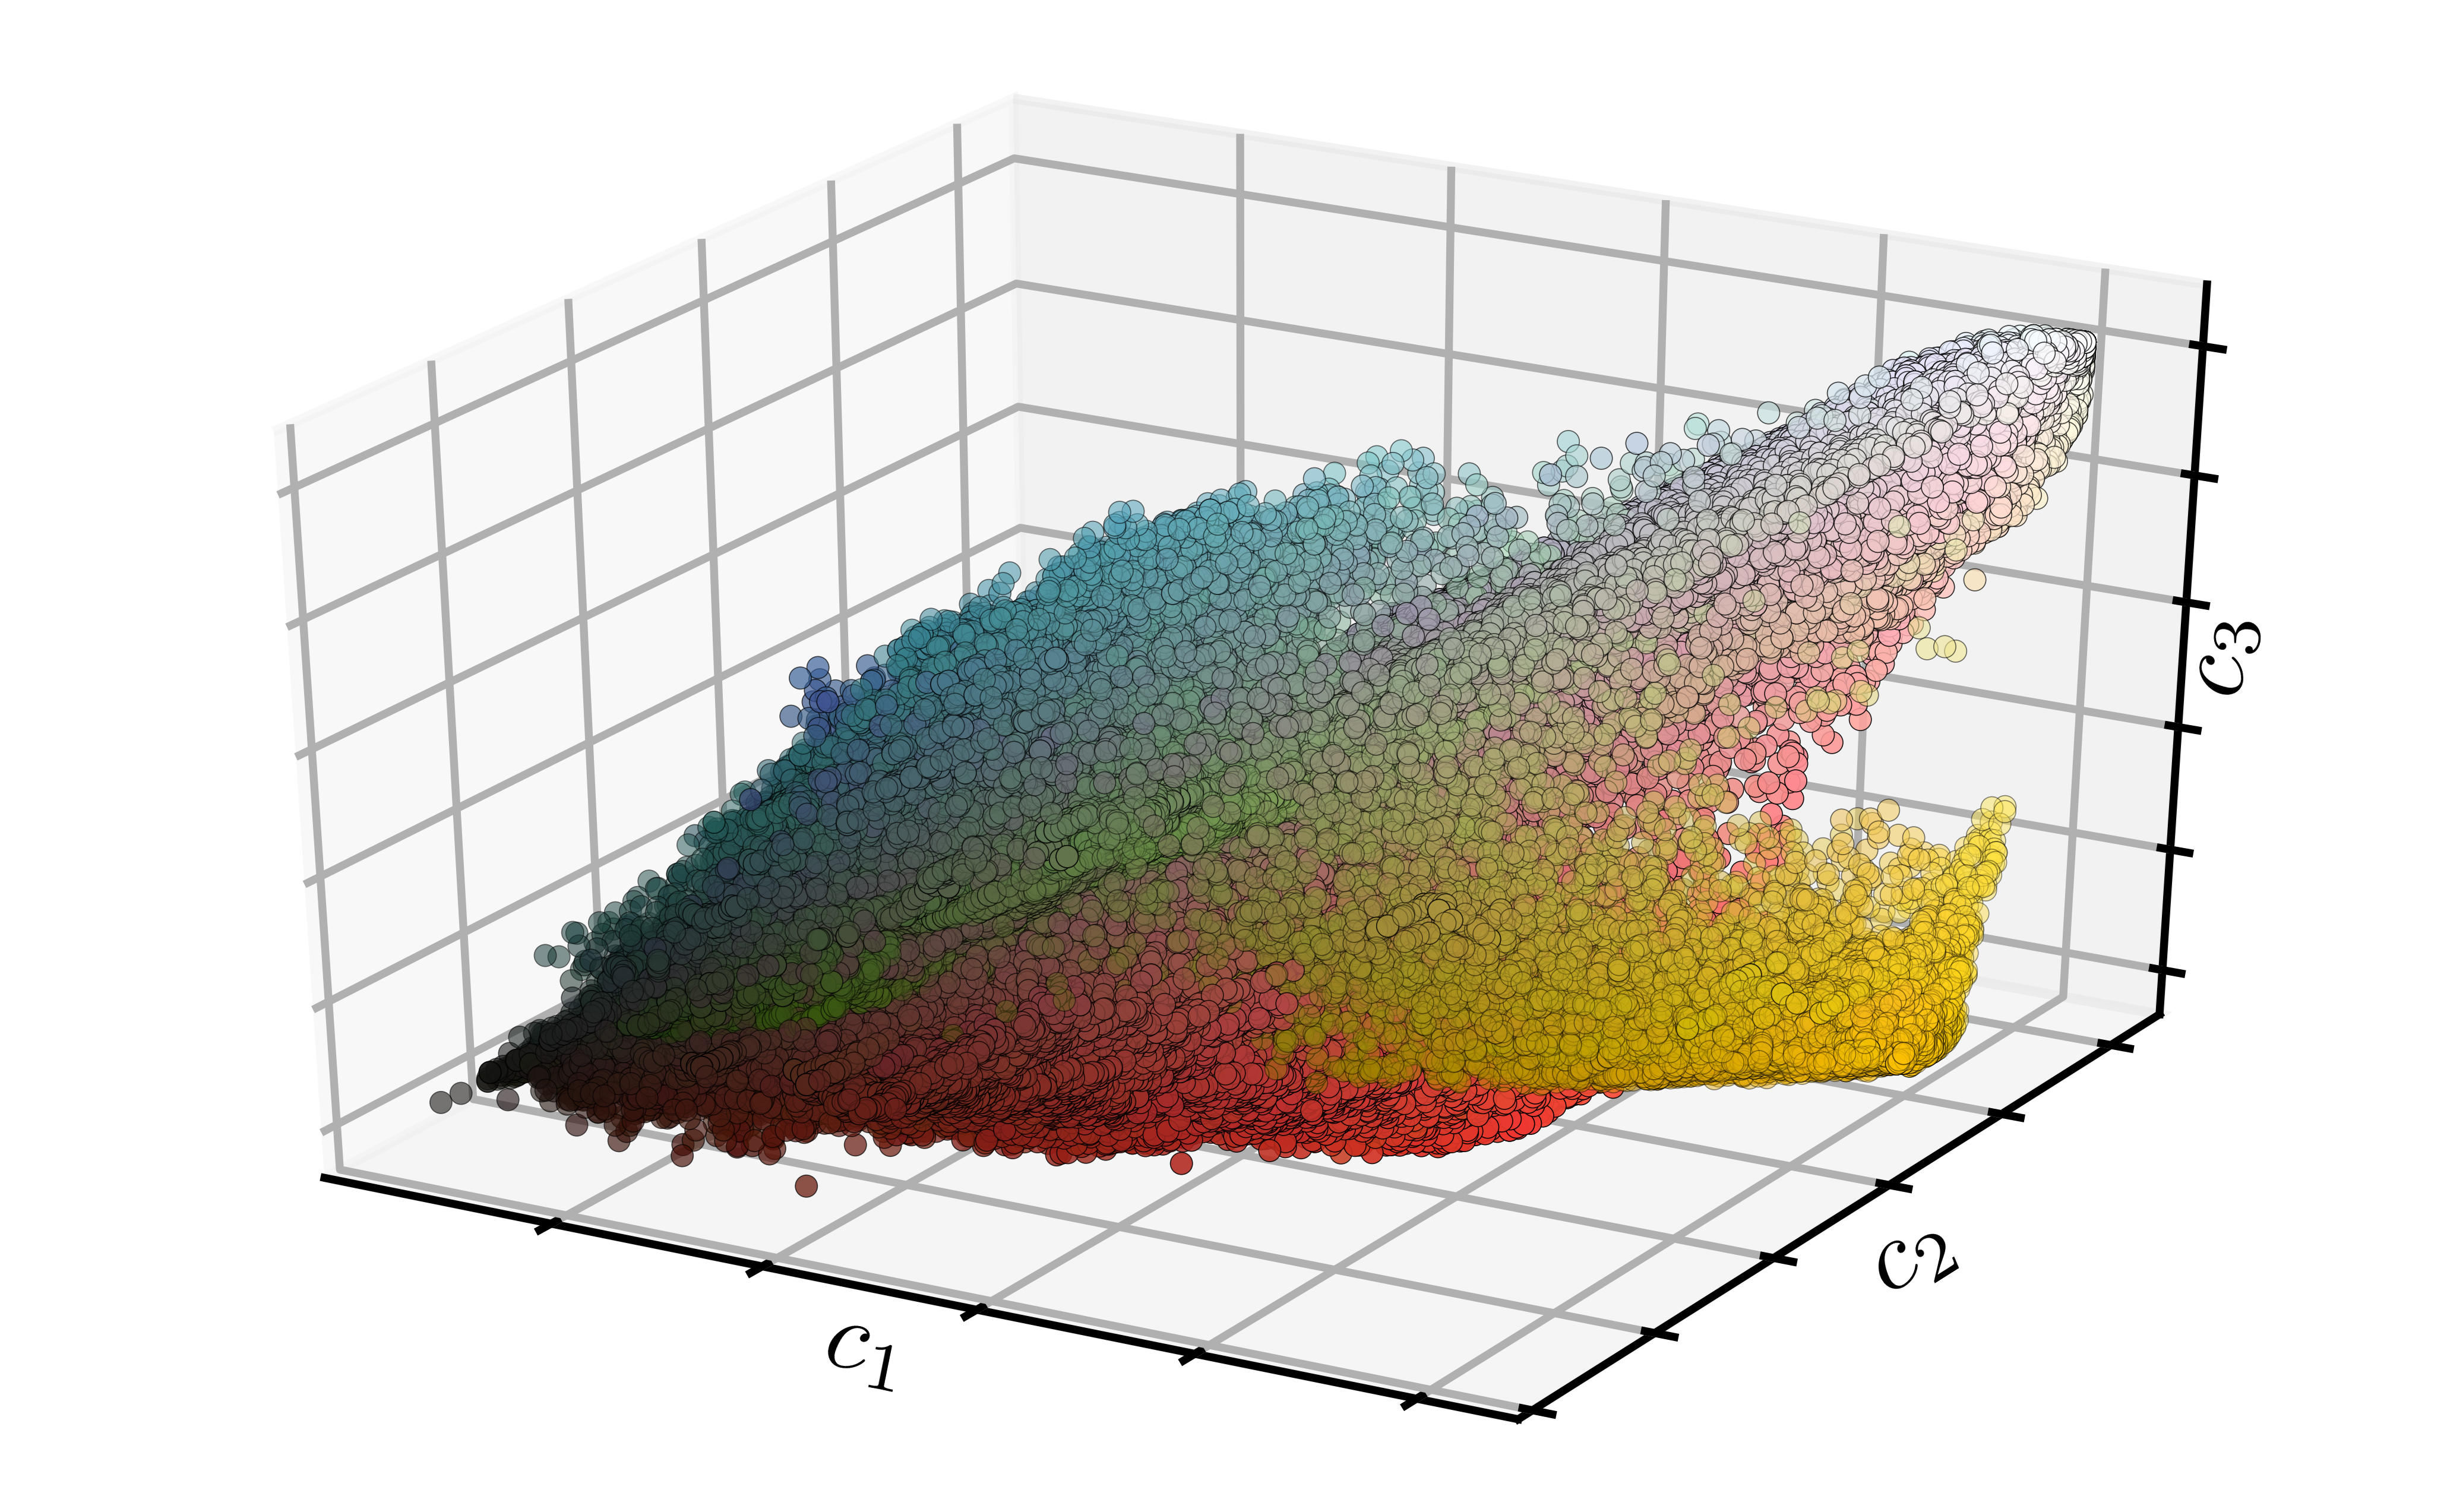
\includegraphics[width=\textwidth]{araras_3d_distribution}
%    \end{subfigure}~
    \begin{subfigure}[b]{0.32\textwidth}
        \includegraphics[width=\textwidth]{clownfish_3d_distribution}
    \end{subfigure}~
    \begin{subfigure}[b]{0.32\textwidth}
        \includegraphics[width=\textwidth]{mountain_3d_distribution}
    \end{subfigure}\vspace{10pt}
    
    \begin{subfigure}[t]{\dimexpr0.32\textwidth+20pt\relax}
    	\makebox[20pt]{\raisebox{40pt}{ \small\textbf{\textsf{(d)}} }}%
    	\includegraphics[width=\dimexpr\linewidth-20pt\relax]{tempo_3d_histogram}
    \end{subfigure}~ 
%    \begin{subfigure}[b]{0.32\textwidth}
%        \includegraphics[width=\textwidth]{araras_3d_histogram}
%    \end{subfigure}~
    \begin{subfigure}[b]{0.32\textwidth}
        \includegraphics[width=\textwidth]{clownfish_3d_histogram}
    \end{subfigure}~
    \begin{subfigure}[b]{0.32\textwidth}
        \includegraphics[width=\textwidth]{mountain_3d_histogram}
    \end{subfigure}\vspace{10pt}
    
    \begin{subfigure}[t]{\dimexpr0.32\textwidth+20pt\relax}
    	\makebox[20pt]{\raisebox{40pt}{ \small\textbf{\textsf{(e)}} }}%
    	\includegraphics[width=\dimexpr\linewidth-20pt\relax]{tempo_3d_signature}
    \end{subfigure}~ 
%    \begin{subfigure}[b]{0.32\textwidth}
%        \includegraphics[width=\textwidth]{araras_3d_signature}
%    \end{subfigure}~
    \begin{subfigure}[b]{0.32\textwidth}
        \includegraphics[width=\textwidth]{clownfish_3d_signature}
    \end{subfigure}~
    \begin{subfigure}[b]{0.32\textwidth}
        \includegraphics[width=\textwidth]{mountain_3d_signature}
    \end{subfigure}\vspace{10pt}
    
    \begin{subfigure}[t]{\dimexpr0.32\textwidth+20pt\relax}
    	\makebox[20pt]{\raisebox{40pt}{ \small\textbf{\textsf{(f)}} }}%
    	\includegraphics[width=\dimexpr\linewidth-20pt\relax]{tempo_color_clusters}
    \end{subfigure}~ 
%    \begin{subfigure}[b]{0.32\textwidth}
%        \includegraphics[width=\textwidth]{araras_color_clusters}
%    \end{subfigure}~
    \begin{subfigure}[b]{0.32\textwidth}
        \includegraphics[width=\textwidth]{clownfish_color_clusters}
    \end{subfigure}~
    \begin{subfigure}[b]{0.32\textwidth}
        \includegraphics[width=\textwidth]{mountain_color_clusters}
    \end{subfigure}\vspace{-5pt}
    
    \begin{subfigure}[t]{\dimexpr0.32\textwidth+20pt\relax}
    	\makebox[20pt]{\raisebox{25pt}{}}%
    	\includegraphics[width=\dimexpr\linewidth-20pt\relax]{tempo_bar_signature}
    \end{subfigure}~ 
%    \begin{subfigure}[b]{0.32\textwidth}
%        \includegraphics[width=\textwidth]{araras_bar_signature}
%    \end{subfigure}~
    \begin{subfigure}[b]{0.32\textwidth}
        \includegraphics[width=\textwidth]{clownfish_bar_signature}
    \end{subfigure}~
    \begin{subfigure}[b]{0.32\textwidth}
        \includegraphics[width=\textwidth]{mountain_bar_signature}
    \end{subfigure}
                    
	\caption{Different representations of color information. {\small \textsf{\textbf{(a)}}} input color image , {\small \textsf{\textbf{(b)}}} single-channel color histogram , {\small \textsf{\textbf{(c)}}} 3-d color distribution , {\small \textsf{\textbf{(d)}}} 3-d color histogram , {\small \textsf{\textbf{(e)}}} 3-d color signature , {\small \textsf{\textbf{(f)}}} color signature clusters .}\label{fig:color_image_representations}    
\end{figure}


\section{Texture}

\section{Texture characterization}

\begin{figure}[!ht]
    \centering
    \begin{subfigure}[b]{0.19\textwidth}
        \includegraphics[width=\textwidth]{brodatz_skin}
        \caption{}
    \end{subfigure}
    %~ %add desired spacing between images, e. g. ~, \quad, \qquad, \hfill etc. 
      %(or a blank line to force the subfigure onto a new line)
    \begin{subfigure}[b]{0.19\textwidth}
        \includegraphics[width=\textwidth]{brodatz_three}
        \caption{}
    \end{subfigure} 
    %~ %add desired spacing between images, e. g. ~, \quad, \qquad, \hfill etc. 
      %(or a blank line to force the subfigure onto a new line)    
    \begin{subfigure}[b]{0.19\textwidth}
        \includegraphics[width=\textwidth]{brodatz_wall}
        \caption{}
    \end{subfigure}
    %~ %add desired spacing between images, e. g. ~, \quad, \qquad, \hfill etc. 
      %(or a blank line to force the subfigure onto a new line)
    \begin{subfigure}[b]{0.19\textwidth}
        \includegraphics[width=\textwidth]{brodatz_vlines}
        \caption{}
    \end{subfigure}
    %~ %add desired spacing between images, e. g. ~, \quad, \qquad, \hfill etc. 
      %(or a blank line to force the subfigure onto a new line)
    \begin{subfigure}[b]{0.19\textwidth}
        \includegraphics[width=\textwidth]{brodatz_sponge}
        \caption{}
    \end{subfigure}\\
    
    \begin{subfigure}[b]{0.19\textwidth}
        \includegraphics[width=\textwidth]{brodatz_tissue}
        \caption{}
    \end{subfigure}
    %~ %add desired spacing between images, e. g. ~, \quad, \qquad, \hfill etc. 
      %(or a blank line to force the subfigure onto a new line)
    \begin{subfigure}[b]{0.19\textwidth}
        \includegraphics[width=\textwidth]{brodatz_cafe}
        \caption{}
    \end{subfigure} 
    %~ %add desired spacing between images, e. g. ~, \quad, \qquad, \hfill etc. 
      %(or a blank line to force the subfigure onto a new line)    
    \begin{subfigure}[b]{0.19\textwidth}
        \includegraphics[width=\textwidth]{brodatz_crystal}
        \caption{}
    \end{subfigure}
    %~ %add desired spacing between images, e. g. ~, \quad, \qquad, \hfill etc. 
      %(or a blank line to force the subfigure onto a new line)
    \begin{subfigure}[b]{0.19\textwidth}
        \includegraphics[width=\textwidth]{brodatz_flowers}
        \caption{}
    \end{subfigure}
    %~ %add desired spacing between images, e. g. ~, \quad, \qquad, \hfill etc. 
      %(or a blank line to force the subfigure onto a new line)
    \begin{subfigure}[b]{0.19\textwidth}
        \includegraphics[width=\textwidth]{brodatz_paint}
        \caption{}
    \end{subfigure}    
                  
    \caption{ Examples of texture images and its classification. [{\small \textsf{\textbf{(a) (b) (e) (h)}}}] nautural textures, [{\small \textsf{\textbf{(c) (d) (f) (g) (i) (j)}}}] man-made textures, [{\small \textsf{\textbf{(c) (d)}}}] regular textures, [{\small \textsf{\textbf{(g) (h)}}}] stochastic textures, [{\small \textsf{\textbf{(c) (d)}}}] homogeneous, [{\small \textsf{\textbf{(a) (b) (f) (g) (h)}}}] weakly-homogeneous, [{\small \textsf{\textbf{(i) (j)}}}] inhomogeneous.}\label{fig:texture_images}    
\end{figure}


\begin{itemize}
	\item Natural and artificial 
	\item Regular, stochastic
	\item Homogeneous, non-homogeneous, in-homogeneous
\end{itemize}



There is a disagreement in the definition of texture in the field of computer vision. It is possible to give a mathematical definition based on its statistical properties, however, these properties are very imprecise and/or restrictive to adapt to the diversity of existing textures.

The definition that we support is based on an experimental finding: a texture is a field of the image that appears as a coherent and homogeneous domain, that is, it forms a whole for an observer. In fact, it is this property of coherence of the texture placed in the context of being perceived as a homogeneous whole for the human eye that is most often sought for image processing, either with the aim of isolating textures, to segment the image or for the recognition of regions.

Some examples of natural textures are shown in the figure. These images come from the reference work Brodatz and show the possible variety of textures that are commonly used to test different algorithms and methods of vision.

The perception of textures is a key property of human vision. Although there is still no generalized definition, we can define texture as a measure of coarseness, contrast, directionality, line similarity, regularity and roughness. Therefore, the features that chracterize texture attempt to capture the granularity and repetition of perceptually similar patterns of surfaces within a region of the image, such that a human observer perceives the region as homogeneous.
Unlike color, texture information is not a purely pixel-level property. Texture implies the notion of spatial extent, that is, that the spatial variation of intensities of a group of pixels generate textures in the images.

There are numerous studies that review, compare and organize the work of texture analysis in different ways \citep{Materka.Strzelecki:Report:1998}, \citep{Zhang.Tan:PR:2002}, \citep{Bharati.Liu.ea:CILS:2004},\citep{Lukashevich.Sadykhov:ICPCI:2012}, \citep{Humeau-Heurtier:IEEEAccess:2019}. One possible organization is based on its operating principle, which classifies the texture characterization techniques into: statistical methods, structural method, model-based methods, transform-based methods, graph-based methods, learning-based methods and entropy-based methods. In this chapter we review five of the most widely used methods in the literature and their techniques for extracting textures fearures.

% \begin{enumerate}[noitemsep]%,topsep=0pt
%	\item Statistical methods
%	\item Structural methods
%	\item Model-based methods
%	\item Transform-based methods
%	\item Graph-based methods
%	\item Learning-based methods
%	\item Entropy-based methods
%\end{enumerate}
%	

\subsection{Statistical Methods}
Statistical methods contemplate that textures are determined by the way the gray levels are distributed over the pixels of an image. In these methods, the gray level distribution of the image is represented by a histogram.

A first approach in this category is the histogram properties analysis \citep{Aggarwal.K.Agrawal:JSIP:2012}. The first-order statistics properties are the mean and the Central Moments of the 1D histogram, that is, the variance, skewness, and kurtosis. These properties provide information on the distribution of the gray levels of the image from a global point of view, taking into account individually the gray level of the pixels. Hoewever, they do not provide any information on how the gray level of a pixel at a given location statistically affects the gray level value of another pixel at a relative location from the reference pixel.
The second-order statistical properties explore this option ang give a description of the texture, based on the comparison of intensity values of two pixels. In this case the Co-Occurrence matrix \citep{Haralick.Shanmugam.ea:TSMC:1973} is the second-level histogram that maps the intensity distribution of the pixels. Some of the texture features extracted from the second-order statistics are Angular Second Moment (ASM), Contrast, Correlation, Homogeneity, Entropy and Energy.

Local Binary Patterns (LBP) \citep{Ojala.Pietikainen.ea:PR:1996} are another technique for obtaining second-level histograms. This approach summarizes the spatial structure and local contrast of an image within a binary pattern, comparing the gray level of each pixel with its neighborhood. If the intensity value of the central pixel is greater than its neighbor, then it is denoted by 1, otherwise by 0. Subsequently, a binary array is constructed, following a consistent ordering of the neighboring values, which is transformed to decimal number and stored in a new array. The process of thresholding, construction of binary strings, binary to decimal transformation, and storing of decimal output is performed for all pixels in the image, resulting in an LPB image. Finally the second-level histogram for texture chraracterization is obtained from this resulting LBP image.

\subsection{Structural Methods}
The structural methods are based on the decomposition of the image in basic units, i.e., in elements, low-level primitives o texels. Such units can be points, lines, regions, or shapes. The basic units and their spatial arrangement in the image are used to characterize the textures. These approaches consider that textures are patterns formed by replication, more or less regular, of a basic unit. The arrangement of the primitives allows obtaining geometric relationships and subsequently statistical properties that serve serve to characterize textures. Structural tecniques aim to determine the textual primitive and define the location rules.

Dpends on the application, structural tecniques differ according to the choice of primitives. Some of the commonly considered primitives are pixels, regions of uniform intensity, line segments, or peaks in the gray level distribution. For the recovery of these primitives, highly known approaches are generally used, for example, the SIFT (Scale Invariant Feature Trasform) operator in the case of characteristic points and the contour detectors, such as Sobel and Canny, for line and edge recovery. On the other hand, the primitive's measurements and statistics most commonly used are intensity, orientation, elongation, curvature, compactness, among others.

\subsection{Model-based Methods}
This group of methods stipulates that the textures can be described by some mathematical model. This category is mainly subdivided into two approaches: stochastics and fractals.

Stochastic methods for texture modeling are very popular, in particular random field models. In this context, a texture model is a parametric family of spatially homogeneous random fields, which depend on a series of hyperparameters \citep{Winkler:Book:2003}. Inside such a family a specific texture can be characterized by a special set of hyperparameters that captures its characteristic features. According to the properties of the random fields, some of the models used for the characterization of texture are Markov Random Field (MRF) \citep{Hassner.Sklansky:CGIM:1980, Cross.Jain:PAMI:1983}, Gibbs Random Field (GRF) \citep{Derin.Cole:CVGIM:1986}, Conditional Random Field (CRF), Gaussian Markov Random Field (GMRF) \citep{Cohen.Fan.ea:PAMI:1991}.

Within the category of stochastic approaches, there is a group of techniques that use probabilistic approaches and mathematical morphology operators for the modeling of random textures \citep{Serra:CGIM:1980}, \citep{Cord.Bach.ea:JoM:2010}.

Fractal models consider textures as complex chaotic systems, so they exhibit fractal behavior. Textures, as fractal objects, have identical shape and statistical characteristics at different scales. Fractal geometry relies on self similarity across multiple scales and is measured with the fractal dimension. Fractal model-based approaches aim to determine fractal dimension, find fractal geometry, and calculate fractal measurements for the description of textures in images.


\subsection{Transform-based Methods}
Transform methods map an image to a space within which the textures are characterizable. The peculiarity is that the new space coordinates allow the interpretation of the textures because they reflect the texture properties, for example, the log-polar coordinates in the case of Gabor transform, they reflect the periodicity and orientation of the textures present in an image.

Within this category, one of the most notable methods for the extraction of texture features are Law's filter banks \citep{Laws:IUW:1979, Laws:IPMG:1980, Laws:Report:1980}. There are also the approaches based on the Fourier transform \citep{Ursani.Kpalma.ea:ICMV:2007}, where it is used to decompose the image into its frequency components. Following the same principle, there are the approaches based on Gabor decomposition \citep{Gabor:JIEE:1946} and those based on wavelets \citep{Arivazhagan.Ganesan:PR:2003}, which analyze the content of a texture not only in the frequency domain, but also in the spatial domain. On the one hand, the Gabor filter is defined as a sinusoidal wave plane modulated Gaussian kernel, which can be adapted in frequency, orientation and bandwidth. For its part, the wavelet transform allows the analysis of the texture in the frequency and spatial domain by means of the dilation and translation, respectively, of a mother wavelet.

\subsection{Learning-based Methods}
The methods for the extraction of texture features based on learning are relatively new with respect to the other methods mentioned in this work.
This category of approaches can be divided into two subclasses: the visual dictionary methods and the deep learning methods.

Visual dictionary methods are motivated by natural language processing algorithms. In this case, the aim is to generate a codebook or dictionary that contains basic geometric elements of the images, also called \textit{textons}. In the document processing analogy, textons correspond to words; so an image can be described by the repetition (organized or not) of a set of textons.

There are different strategies for calculating textons \citep{Zhu.Guo.ea:IJCV:2005}. For example, the approaches based on generative models, where an image is considered to be a linear combination of some base images. Such base images are represented by Gabor or Laplacian-of-Gaussian (LoG) functions and other wavelet transforms. Following the principle of generative models, textons are the base functions learned from a large number of image patches.
Other approaches to obtaining textons are based on discriminative modeling. In this case, the base functions are rotated and scaled filters that form a family which is convolved with the image. The responses of the filters form a feature space  in which it is possible to form clusters. Each cluster center then corresponds to a texton. To obtain a texton dictionary, it is necessary to obtain the feature space and the cluster centers from a group of training images.

Models based on deep learning use Convolutional Neural Networks (CNNs) for the extraction and representation of image features. CNNs consist of multiple locally connected layers which covolve kernels over the entire image. These approaches analyze the information of a group of images to generate a model. The characteristics of the learned model are a function of the input images, which in the case of the study of texture, is expected to generalize the properties of granularity, frequency, orientation, etc. of patterns in the training dataset.


%\section{Conclusions}

